\chapter{Design}
\label{ch:design}

In this chapter we will design the data structure of our test data,
as well as the workloads to simulate a typical industrial use of a database.

After that we will plan our extension for YCSB in section~\ref{ch:design:se:extensionOfTheBenchmark},
both for the internals of the benchmark and the bindings to connect the databases with the benchmark.

At the end in section~\ref{ch:design:se:executionTool} and~\ref{ch:design:se:evaluationTool} we will outline tools to support execution of the benchmark and evaluation of the results.

\section{Data Structure}
\label{ch:design:se:dataStructure}
To design a schema for our data structure we had a meeting with other researchers at our institute.
The result of our session can be seen in figure~\ref{fig:firstDesignOfSchema}.
In the centre left we see "Features of Interest" which could be mapped to the "testFeature" edge in the industrial example of figure~\ref{fig:exampleData} as it depicts an observation of a product.
At the bottom we see a "M" which stands for "Machine",
its connection to "P. Schritte"\footnote{german for production steps} shows that this machine does \texttt{1} to \texttt{n} production steps.
Every production step is associated with a component which consists of a PCB\footnote{short for printed circuit board} that has different parts,
a version and a file after which it was created.

As the model shows too much detail in some areas without giving a good overview of an industrial data schema,
we had to reiterate over it and get rid of some complexity where we don't need it for our purposes.

\begin{figure}
  \centering
  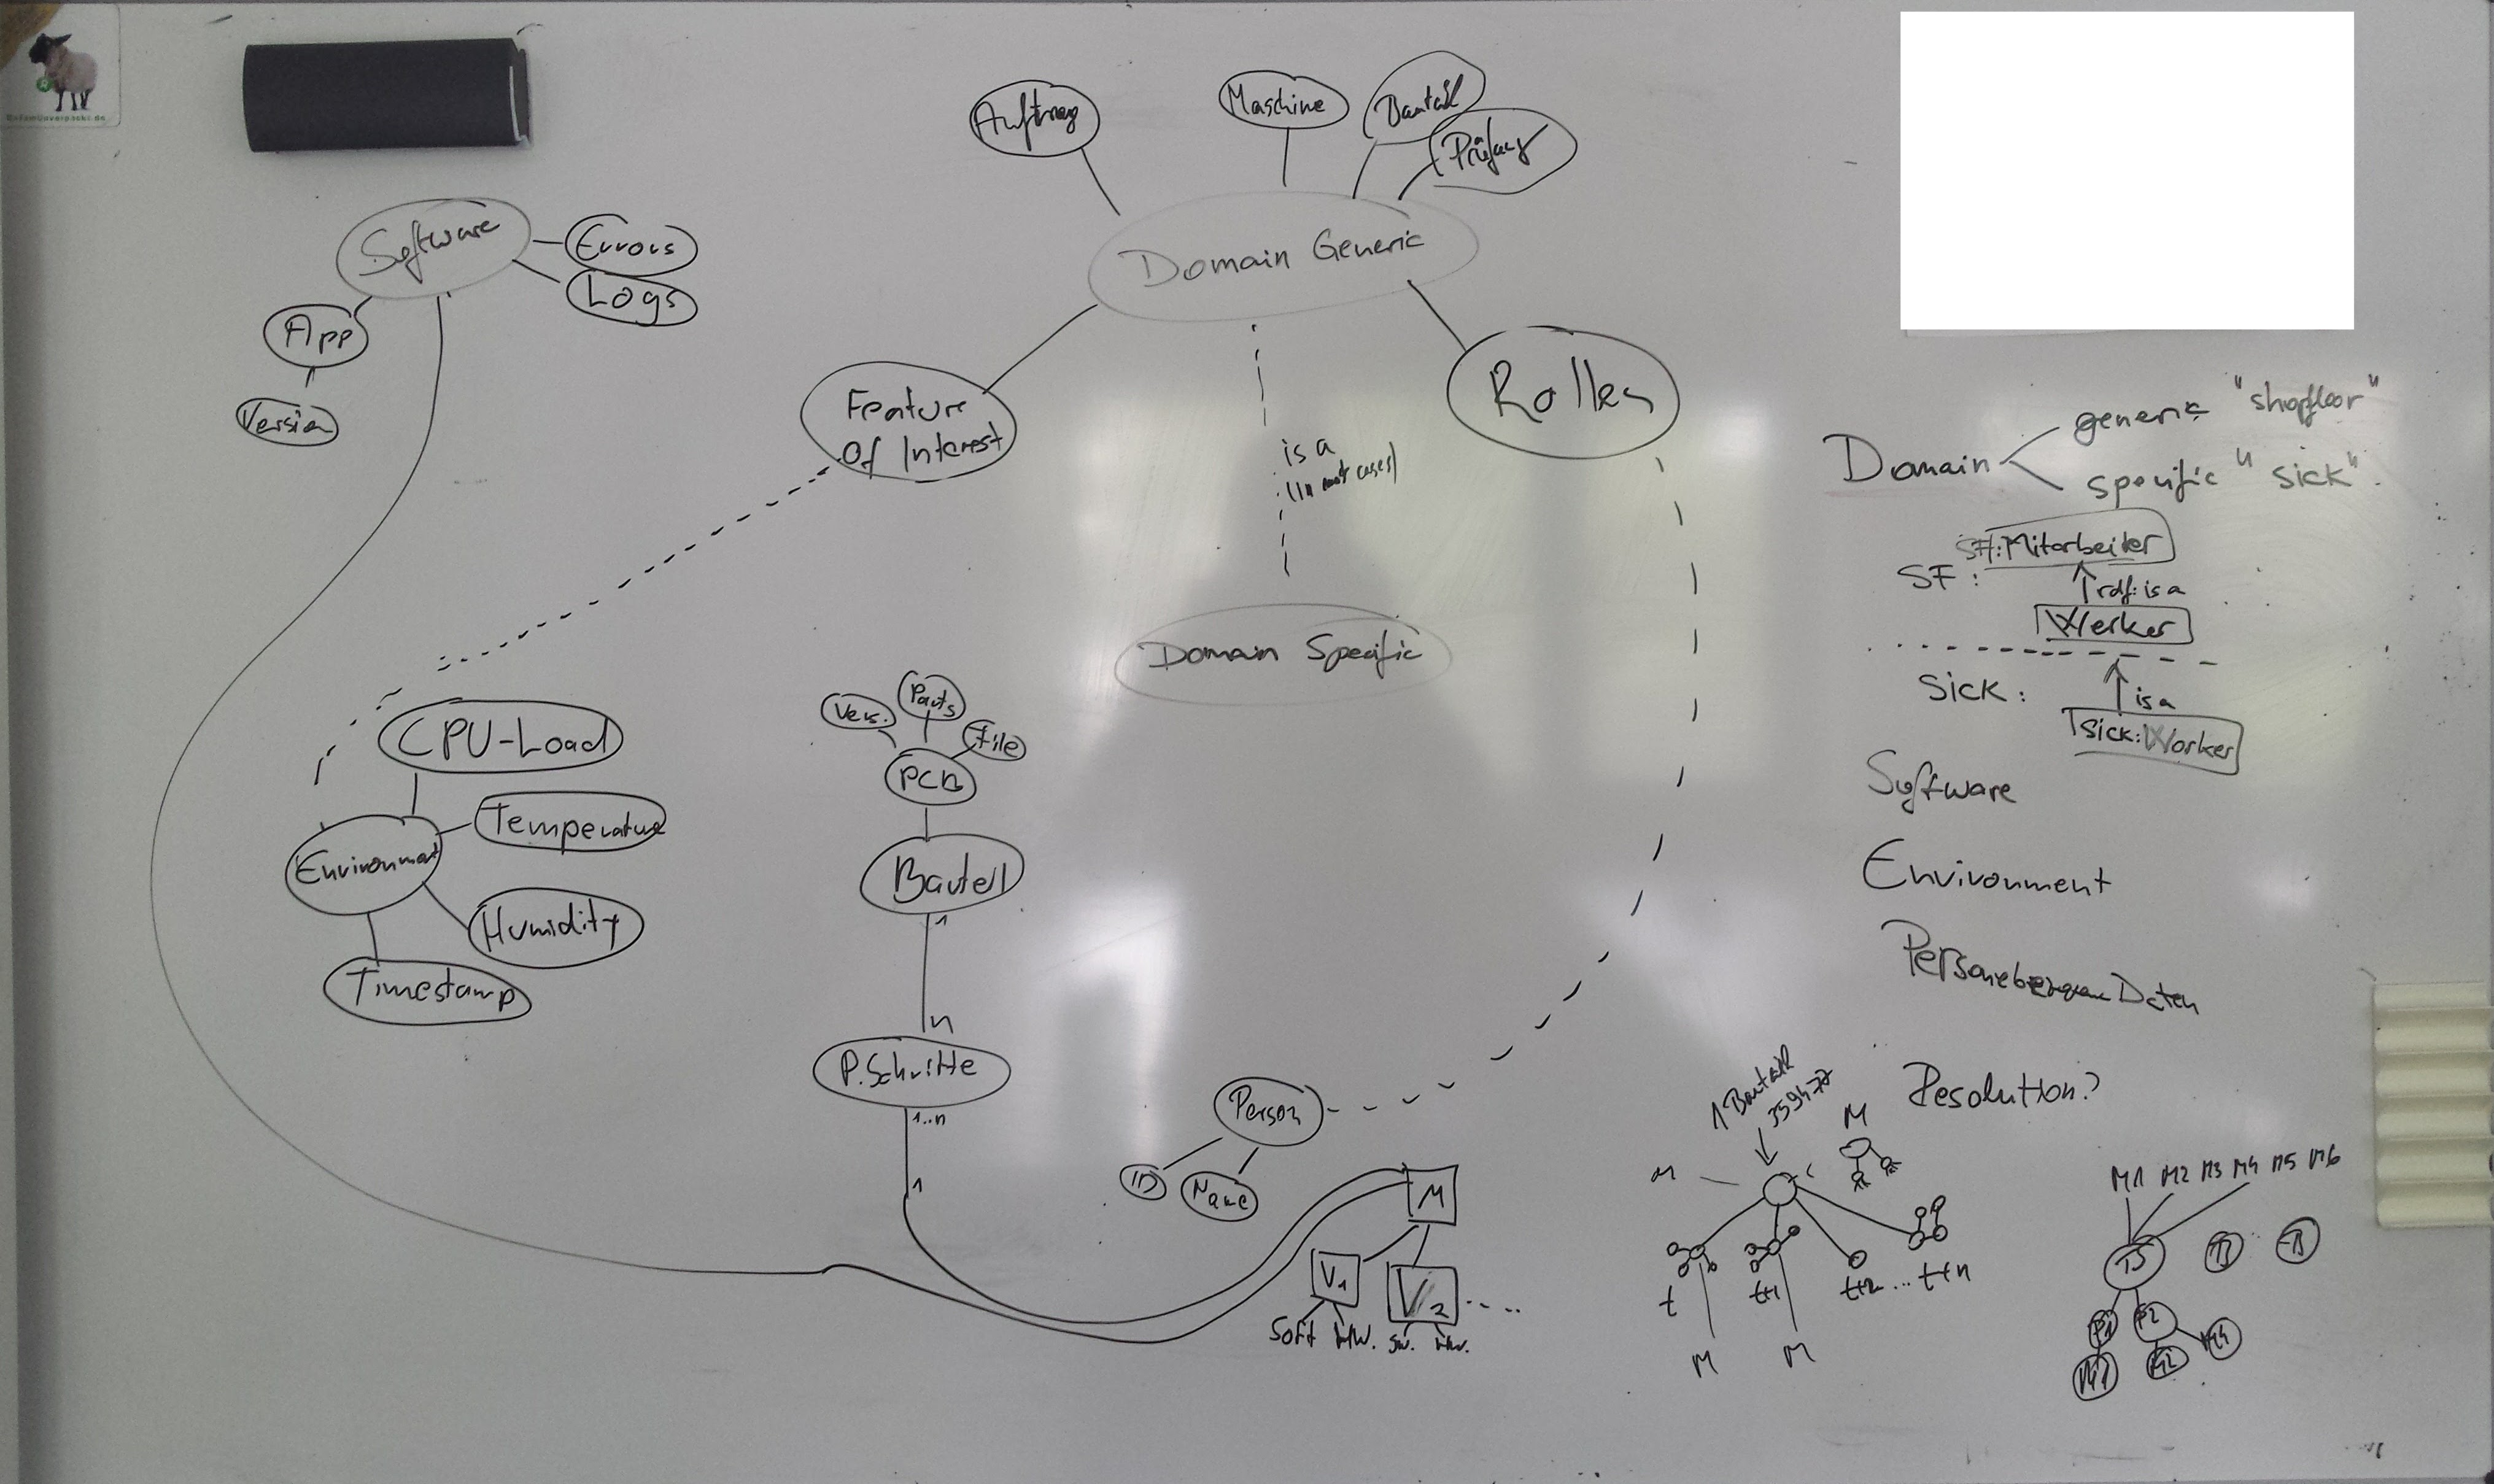
\includegraphics[width=\textwidth]{images/design/firstDesignOfSchema}
  \caption{The first design of a data schema for industrial data. Created by researchers at our institute.}
  \label{fig:firstDesignOfSchema}
\end{figure}

The meeting gave us a better understanding of how a production facility could handle its data and with that in mind and the objective to design a simpler schema that includes to most necessary parts of production the model shown in figure~\ref{fig:finalDesignOfSchema} was created. \\
At the top is the \texttt{Factory},
which has an \texttt{Orders} node that represents the folder for all \texttt{Order}s received by the \texttt{Factory}.
A \texttt{Machine} and a \texttt{Design} are linked to the \texttt{Factory},
these represent the production machine and the design template for products made by that machine.
A \texttt{Product} has incoming edges from the \texttt{Design} it is made after, the \texttt{Machine} it was produced by and the \texttt{Order} for which it is created.
Variable \texttt{x} determines how many \texttt{Product}s are made for each \texttt{Order}.
The \texttt{Product} was made at a specific \texttt{Date} and consists of one or multiple \texttt{Component}s depending on the value of variable \texttt{y}.
Every \texttt{Component} undergoes a test suite (\texttt{Tests}) which contains of a number of \texttt{Test Parameter}s,
which number is defined by \texttt{z}.\\
For easier reference we will call \texttt{x} productsPerOrder, \texttt{y} componentsPerProduct and \texttt{z} testParameterCount.

\begin{figure}
  \centering
  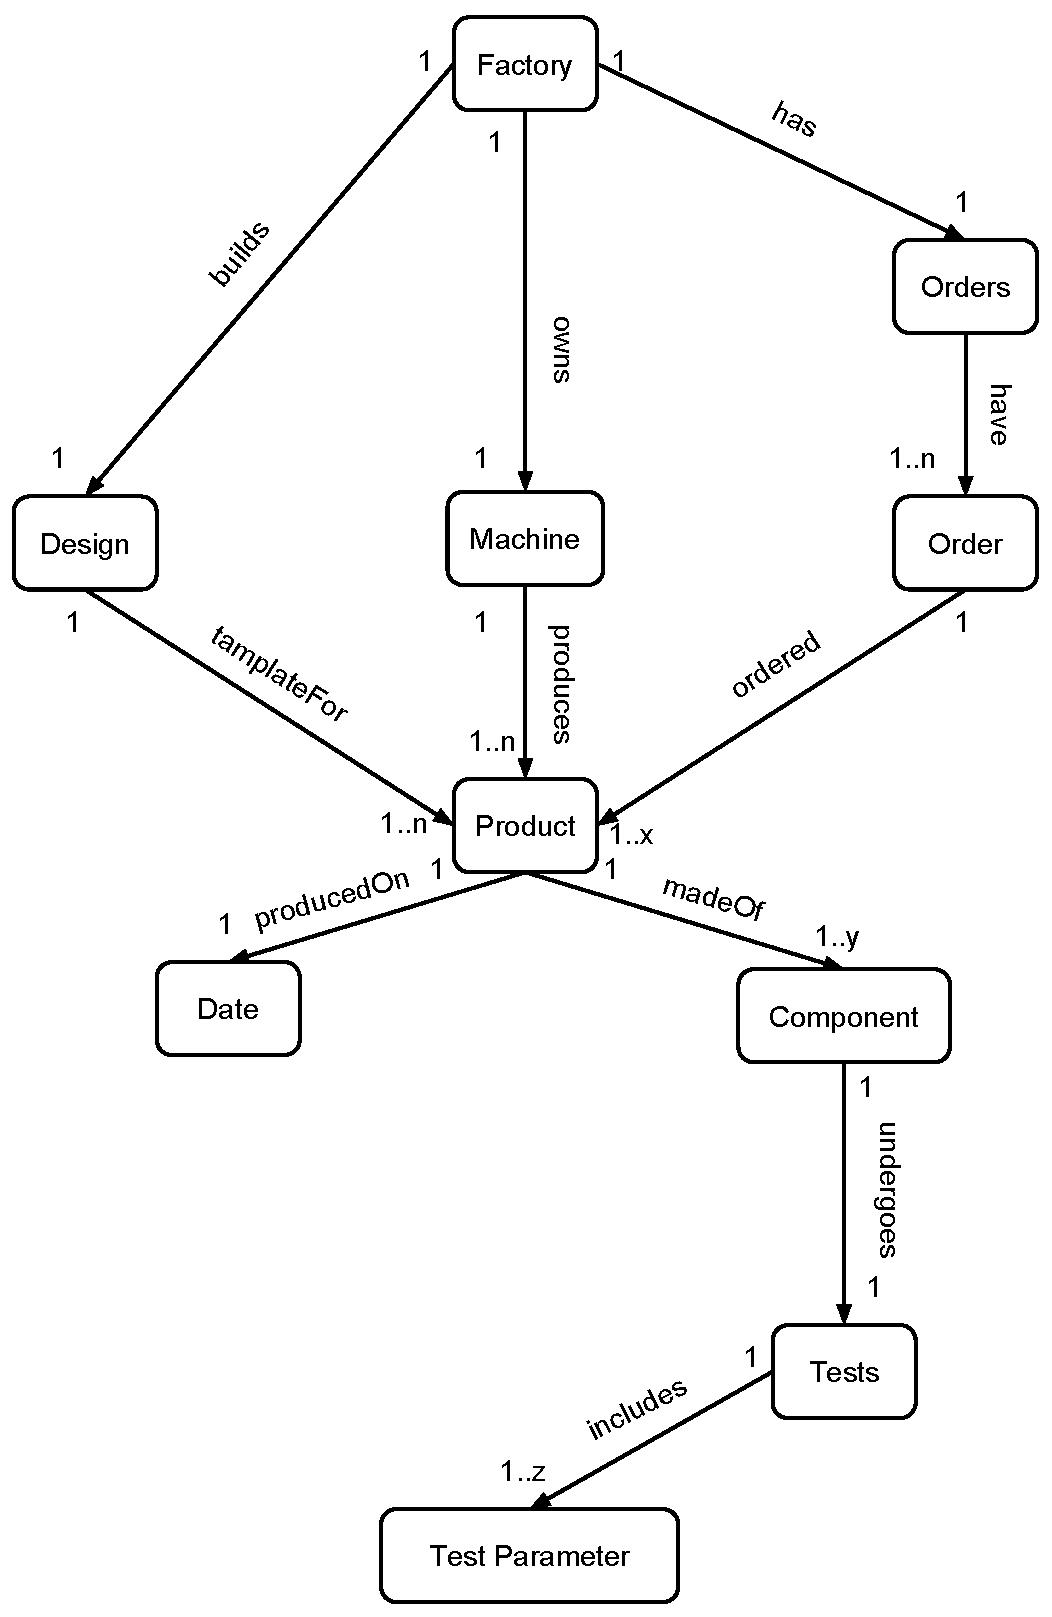
\includegraphics[width=.75\textwidth]{images/design/dataStructure}
  \caption{The final design of the data schema.}
  \label{fig:finalDesignOfSchema}
\end{figure}

\section{Workloads}
\label{ch:design:se:workloads}
Our workload design will be separated into three parts.
In subsection~\ref{ch:design:se:throughput} we discuss the design of workloads aimed to reveal the ability to store large amounts of data.
Subsection~\ref{ch:design:se:productionSimulation} will investigate the suitability of a database to be used in an industrial use case for storing data.
We will design workloads to examine how well the databases can retrieve data under load in subsection~\ref{ch:design:se:retrievingUnderLoad}.
Finally,
we will give a summary over all workloads we are going to run on the databases in subsection~\ref{ch:design:se:summary}

\subsection{Throughput}
\label{ch:design:se:throughput}
To explore the throughput of the databases we will change some variables over the course of the different workloads.
These variables are

\begin{itemize}
  \item using an index on the key
  \item the size of a single property of the node
  \item using no edges.
\end{itemize}

The last variable sounds counter intuitive,
since edges add meaning to the data,
but by eliminating them we want to see if edges could be a cause of delay,
because to add an edge the start and end node need to be known and therefore be retrieved at first.

We will go over the different variables in the following subsections and motivate their purpose.

\subsubsection{Index}
\label{ch:design:se:index}
For this category we will use different dataset sizes in terms of their number of nodes.
We will use steps of multiplication by 10 from 1000 nodes to 10000000 nodes,
to examine if the throughput changes,
as the database is filled with data.

Switching from indexed to not indexed we want to inspect how the throughput is effected by not using an index.
Indexing is important to retrieve data more quickly for the cost of write speed.
With this workload we will see if there is a sacrifice in write throughput,
as to store an edge,
two nodes have to be looked up.
We will only use an index on the node and edge key,
which will be used to search that graph component\footnote{a node or an edge of the graph} in the database.
Indexing the other properties would have no benefit in our example.

For this workload we will use a node property size of 10B.
That is small enough to not have an impact on performance but large enough to represent most of the data stored in the properties of our example.

\subsubsection{Node Property Size}
\label{ch:design:se:nodePropertySize}
After retrieving the number of nodes that represents an acceptable execution time,
we will vary the next variable which is the property size.
We will go from 10B used in the index benchmarks to up to 1MB,
again in steps of multiplying by 10 (10B, 100B, 1KB, ..., 1MB).
We want to examine if there is a drawback for throughput when storing more information in the nodes and at which point the size is too large.

The typical property size is between 1B (1 character) and roughly 75B (75 characters) according to our example in listing~\ref{lst:exampleData}.

The use of properties isn't limited to short strings,
that is why we will investigate if larger amounts of data influence the throughput more than linearly.

We will use an index on the keys,
because that represents the use in the industry and since we aren't indexing the growing values there will be no impact from using it.

\subsubsection{No Edges}
\label{ch:design:se:noEdges}
In subsection~\ref{ch:design:se:throughput} we already justified why we will investigate the throughput with an exclusive use of nodes in the dataset.
To summarise,
the use of this workload is to see if there is a big difference in using edges and therefore determine how the e/n ratio effects the throughput.

As in subsection~\ref{ch:design:se:nodePropertySize} we will use a suitable large dataset in terms of node count resulting from the first workloads.
We will use the same node size as in~\ref{ch:design:se:index} and an index to be able to compare the result directly to the corresponding one from that workload.

\subsection{Production Simulation}
\label{ch:design:se:productionSimulation}
Related to production we will investigate the impact of the structure and the general suitability for an industrial use.
The next two subsections will cover those aspects in more detail.

The property size will be set to 50B,
which should be enough to cover on average most values stored in the database.

\subsubsection{Structure}
For production we have some variables to investigate,
which affect the structure of our data and the e/n ratio.
We have three layers which we can scale up horizontally by increasing the corresponding parameters,
which are

\begin{itemize}
  \item productsPerOrder, this spreads the data graph apart at a level closer to the root
  \item componentsPerProduct, this changed the width in the middle of the graph
  \item testParameterCount, which widens the graph at the lowest level.
\end{itemize}

For production simulation we will first examine if the data structure impacts performance of the databases.
To investigate this aspect,
we will change the width of the graph with the variables mentioned above.
We will use the numbers from section~\ref{ch:analysis:se:data} as the maximum width,
which would be \texttt{productsPerOrder = 64},
\texttt{componentsPerProduct = 128} and \texttt{testParameterCount = 128}.
In the first workload we will set all variables to one,
the next one will use \texttt{productsPerOrder = 16},
\texttt{componentsPerProduct = 32} and \texttt{testParameterCount = 32}.
The third and last one will use the maximum width mentioned above.
By this variation we will cover the minimum and maximum with an additional result in the middle to see if there are any changes in performance.

The keys of the graph components will be indexed,
because indexing these values should be done to later work on that data more efficiently,
which is necessary for the industry.

\subsubsection{Suitability}
\label{ch:design:se:suitability}
To examine whether a database is suitable for the industry it should be able to store the data faster than it is coming from the machines.
In section~\ref{ch:analysis:se:dataAmount} we calculated that 1056833 nodes would be written to the database every three minutes.

Now that we have our data structure we can calculate how many edges are contained in that graph and finally how many inserts have to be performed every second.
We will count the incoming edges for every node and also use the variables \texttt{x}, \texttt{y} and \texttt{z} from the structure in~\ref{ch:design:se:dataStructure}.

\begin{equation}
  \label{eq:dataEdges}
  \begin{aligned}
    n_{edges} &= n_{Order} + 3 \times n_{Product} + n_{Product} \\
    &\quad \times (n_{Date} + n_{Component} \times (n_{Tests} + n_{TestParameter})) \\
    \iff &= 1 + 3 \times x + x \times (1 + y \times (1 + z)) \quad | \quad x = 64, y = 128, z = 128 \\
    \implies &= 1 + 3 \times 64 + 64 \times (1 + 128 \times (1 + 128)) \\
    \iff &= 1 + 192 + 64 \times (1 + 128 \times 129) \\
    \iff &= 1 + 192 + 64 \times (1 + 16512) \\
    \iff &= 1 + 192 + 64 \times 16513 \\
    \iff &= 1 + 192 + 1056832 \\
    \iff &= 1057025
  \end{aligned}
\end{equation}

Together with the number of nodes we can calculate the total amount of elements being inserted into the database,
as shown in equation~\ref{eq:dataElements}.

\begin{equation}
  \label{eq:dataElements}
  \begin{aligned}
    n_{total} &= n_{nodes} + n_{edges} \\
    \iff &= 1056833 + 1057025 \\
    \iff &= 2113858
  \end{aligned}
\end{equation}

To convert that into our target throughput we divide that number by three minutes.

\begin{equation}
  \label{eq:dataElements}
  \begin{aligned}
    n_{target} &= n_{total} \times \frac{1}{3 \times 60s} \\
    \iff &= 2113858 \times \frac{1}{180s} \\
    \iff &= 11743,66 \frac{1}{s}
  \end{aligned}
\end{equation}

First,
we will set up a dataset with that number of nodes and insert it into the database.
That will allow us to compare the time needed to store all data with our three-minute limit.
If the database should take more than three minutes,
it wouldn't be suitable,
since data is produced faster than it can be stored.

We will use the structure with the maximum width,
because it represents the industrial use case the best regarding the information given by our partners at SICK AG~\cite{SICK}.

\subsection{Retrieving under load}
\label{ch:design:se:retrievingUnderLoad}
There would be no point in storing data if it isn't retrieved at some point.
To investigate the performance of reading and scanning (more on that in subsection~\ref{ch:design:se:scanning}) data from the database,
the following workloads are designed.

As mentioned in section~\ref{ch:design:se:index} indexing is important for retrieving data,
therefore we will use it as a variable for this workload category.
By doing so we want to examine if the price we pay while writing is justified by the performance gain in retrieving data.

The node amount will be determined by the first workload investigating the throughput,
to not take up too much time testing these features.

We want to retrieve both nodes and edges,
because either could be useful,
since the edges also can have informations stored in them.

\subsubsection{Reading}
\label{ch:design:se:reading}
Reading single values is the basic operation when it comes to retrieving data from a database.
Since the database will be under constant load,
because of production delivering data all the time,
we will use $ 5\% $ of the total operations executed in this workload for read operations,
the rest will be insert operations.

\subsubsection{Scanning}
\label{ch:design:se:scanning}
Scanning a graph can be done in multiple ways,
one of them is depth first search~\cite{Tarjan1972},
to retrieve values associated with connected nodes.
For example,
you could start scanning from a machine to get the test features of its produced products.

As in subsection~\ref{ch:design:se:reading} we will use a mix of $ 5\% $ scan operations and $ 95\% $ insert operations,
to simulate the constant load present in an industrial environment.

The number of steps to do during scanning will be $ 1000 $ as that was the default value set in YCSB and it should also represent a good amount of data to read.

\subsection{Summary}
\label{ch:design:se:summary}
In this subsection we will give an overview over all workloads and their variables.

For the workloads measuring the throughput \texttt{productsPerOrder},
\texttt{componentsPerProduct} and \texttt{testParameterCount} will all be set to $ 1 $.
Their overview is shown in table~\ref{tab:throughput}

\begin{table}[!h]
  \begin{minipage}{\textwidth}
    \begin{tabularx}{\textwidth}{ | X | X | X | X | X | }
      \hline
      Aspect & Node Count & Node Size & Index & Only Nodes \\ \hline
      1. With Index & 1000 & 10B & True & False \\ \hline
      2. With Index & 10000 & 10B & True & False \\ \hline
      3. With Index & 100000 & 10B & True & False \\ \hline
      4. With Index & 1000000 & 10B & True & False \\ \hline
      5. With Index & 10000000 & 10B & True & False \\ \hline
      1. Without Index & 1000 & 10B & False & False \\ \hline
      2. Without Index & 10000 & 10B & False & False \\ \hline
      3. Without Index & 100000 & 10B & False & False \\ \hline
      4. Without Index & 1000000 & 10B & False & False \\ \hline
      5. Without Index & 10000000 & 10B & False & False \\ \hline
      1. Node Size & x & 100B & True & False \\ \hline
      2. Node Size & x & 1KB & True & False \\ \hline
      3. Node Size & x & 10KB & True & False \\ \hline
      4. Node Size & x & 100KB & True & False \\ \hline
      5. Node Size & x & 1MB & True & False \\ \hline
      1. No Edges & x & 10B & True & True \\ \hline
    \end{tabularx}
  \end{minipage}
  \caption{Workloads to investigate the throughput. x is a placeholder for a suitable dataset size in terms of execution time.}
  \label{tab:throughput}
\end{table}

The workloads to investigate the suitability for the industry are shown in table~\ref{tab:productionSimulation}.
For these workloads the property size is fixed to 50B and an index is used on all workloads.
Edges are also used in these workloads to reflect the use in the industry.

\begin{table}[!h]
  \begin{minipage}{\textwidth}
    \begin{tabularx}{\textwidth}{ | X | X | X | X | X | }
      \hline
      Aspect & Node Count & products\-Per\-Order & components\-Per\-Product & test\-Parameter\-Count \\ \hline
      1. Structure & x & 1 & 1 & 1 \\ \hline
      2. Structure & x & 16 & 32 & 32 \\ \hline
      3. Structure & x & 64 & 128 & 128 \\ \hline
      1. Suitability (three minutes) & 1056833 & 64 & 128 & 128 \\ \hline
      2. Suitability (hour) & 21136660 & 64 & 128 & 128 \\ \hline
      3. Suitability (day) & 507279840 & 64 & 128 & 128 \\ \hline
      4. Suitability (week) & 3550958880 & 64 & 128 & 128 \\ \hline
      5. Suitability (month) & 15218395200 & 64 & 128 & 128 \\ \hline
      6. Suitability (year) & 185157141600 & 64 & 128 & 128 \\ \hline
    \end{tabularx}
  \end{minipage}
  \caption{Workloads to simulate production. Again, x represents a placeholder for a suitable dataset size.}
  \label{tab:productionSimulation}
\end{table}

The remaining workloads to examine the ability to retrieve data,
are shown in table~\ref{tab:retrievingUnderLoad}.
These workloads will use an appropriate dataset size regarding execution time and a property size,
as in the production simulation,
of 50B.
A simple structure is used to investigate the basic capabilities of data retrieval,
that means \texttt{productsPerOrder},
\texttt{componentsPerProduct} and \texttt{testParameterCount} are set to $ 1 $.

\begin{table}[!h]
  \begin{minipage}{\textwidth}
    \begin{tabularx}{\textwidth}{ | X | X | X | X | X | }
      \hline
      Aspect & Index & Insert Proportion & Read Proportion & Scan Proportion \\ \hline
      1. Reading & True & 95\% & 5\% & 0\% \\ \hline
      2. Reading & False & 95\% & 5\% & 0\% \\ \hline
      1. Scanning & True & 95\% & 0\% & 5\% \\ \hline
      2. Scanning & False & 95\% & 0\% & 5\% \\ \hline
    \end{tabularx}
  \end{minipage}
  \caption{Workloads to investigate capability to retrieve data under load.}
  \label{tab:retrievingUnderLoad}
\end{table}

\pagebreak

\section{Extension of the Benchmark}
\label{ch:design:se:extensionOfTheBenchmark}
To be able to execute the introduced workloads and use the data structure designed above,
we need to extend the YCSB benchmark.
For the benchmark to be able to execute our workloads the way we want them to be executed the following parts of the benchmark need to be extended

\begin{itemize}
  \item Generation of the dataset
  \item Generation of random graph components
  \item Generation of an operation order
  \item Workload to use the generated dataset
  \item Database bindings.
\end{itemize}

In the following subsections we will go in more detail over the different areas we are planning to modify.

\subsection{Graph Data Generator}
YCSB doesn't include a graph data generator,
therefore we need to create one that fulfils our needs.

The generator should create a dataset with the structure mentioned in section~\ref{ch:design:se:dataStructure} and store the data for future reproduction when using the benchmark with the next database.

The two parts of the generator,
one that creates and stores the data and one that recreates the data,
are designed in subsection~\ref{ch:design:se:storingTheDataset} and~\ref{ch:design:se:restoringTheDataset} respectively.

Generally,
to represent a graph in YCSB we need some classes to represent nodes, edges and the graph.
In section~\ref{ch:background:se:graphs} we mentioned that a graph is a tuple of a set of nodes and a set of edges.
That can be directly mapped to a class with two lists,
one for nodes and the other one for edges.
We want the nodes to have a key for identification,
a label to match it with an object that could exist in the real world and a value,
which will represent the data stored in the node.
The size of this value should be directly linked to the property size from~\ref{ch:design:se:nodePropertySize}.
An edge should also have a key for identification,
a label to add meaning to it and a start and an end node,
represented by their identification keys.

The generator of the dataset should decide whether it should create a new one or recreate the dataset,
by looking at the existing files.

\subsubsection{Storing the Dataset}
\label{ch:design:se:storingTheDataset}
We want to control the size of the dataset with our variables mentioned in the workload section~\ref{ch:design:se:workloads} so this generator should create small subgraphs with only one node and its corresponding edges every time it is called for a new value.
By storing the current state of the created graph in the generator class,
we can always determine the next subgraph to create.

The modify the structure of the graph with our three variables,
these need to be passed into this class and used during subgraph creation.

To restore that data also one node at a time we will store each created subgraph in a file,
for that we will serialise the graph and deserialise it when we are restoring the data.

To disable edges for the workload from subsection~\ref{ch:design:se:noEdges} we can simply skip the step of creating and adding them to the graph.

\subsubsection{Restoring the Dataset}
\label{ch:design:se:restoringTheDataset}
The recreation of the data should be easily accomplishable by deserialising it from the created file during creation of the dataset.
Since the single subgraphs were stored in the file,
we can pass them to the workload directly after deserialising them.

To avoid memory issues with larger datasets the subgraphs shouldn't be read all at the beginning but rather on demand,
by deserialising only one line when called.

\subsection{Random Graph Component Generator}
Reading and scanning operations require a point to start with in the data,
that's why we need the key of some component in the graph.
The kay can be randomly chosen,
but the node or edge associated with it has to be present in the database.
Therefore,
we need to somehow store the keys of the graph components we have already inserted into the database.
That could be done in the \texttt{GraphDataGenerator} mentioned in subsection~\ref{ch:design:se:storingTheDataset},
because it touches all generated components anyways.

Because we want to retrieve edges and nodes randomly we have to pick the kind of graph component randomly every time it is required.
As in~\ref{ch:design:se:storingTheDataset} and its subsections,
every created value needs to be stored to be retrieved later on.
The data needed for this generator isn't as complex as a graph and can therefore be stored directly in a file line by line for easy storing and restoring.
That also means,
that we can read the files at the beginning of the run,
so it is more quickly accessible during the benchmark without using too much memory.

For the workload which requires the absence of edges a method should be defined to return only a randomly chosen node.

Figure~\ref{fig:randomGraphComponentGenerator} shows an activity diagram of the generator returning a random graph component.

\begin{figure}
  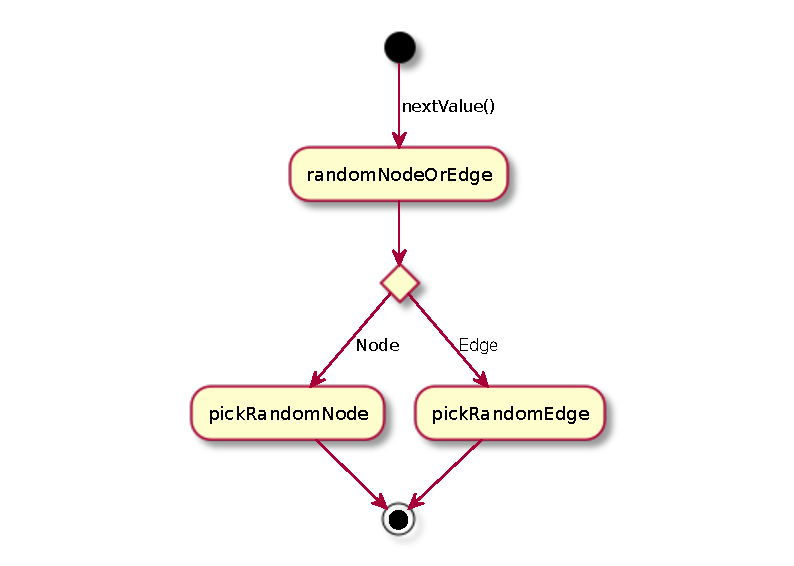
\includegraphics[width=\textwidth]{images/extensions/randomGraphComponentGenerator}
  \caption{Activity diagram of the \texttt{RandomGraphComponentGenerator}, showing the process of storing and restoring a random graph component.}
  \label{fig:randomGraphComponentGenerator}
\end{figure}

\subsection{Operation Order Generator}
\label{ch:design:se:operationOrderGenerator}
To fix the execution order of inserting and retrieving data to and from the graph,
we need to save the operations too.
That can be done by simply storing the name of each operation in a file as it appears and reading it from there when running the benchmark.

In YCSB there is already a \texttt{DiscreteGenerator}\footnote{com.yahoo.ycsb.generator.DiscreteGenerator} that takes pairs of weights and values and returns,
distributed according to the weights,
a value.
This can be used to get the operations to run on the database.

Figure~\ref{fig:operationOrderGenerator} visualises the procedure to return the next operations.

\begin{figure}
  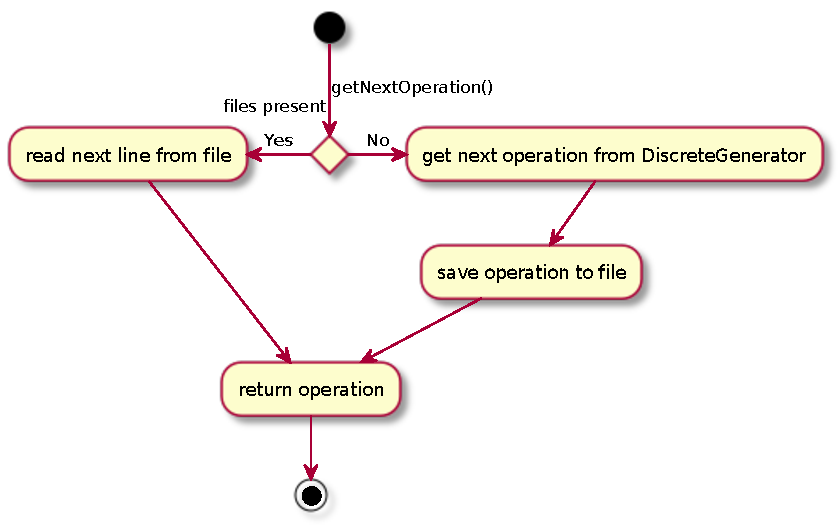
\includegraphics[width=\textwidth]{images/extensions/OperationOrderGenerator}
  \caption{Activity diagram of the \texttt{OperationOrderGenerator::getNextOperation}.}
  \label{fig:operationOrderGenerator}
\end{figure}

\subsection{Graph Workload}
The \texttt{GraphWorkload}s task is to coordinate the different generators and to execute the workload as specified.
To be able to store the generated dataset in a specific folder on the system the workload class should take a path to a folder and instrument the generators to store their data in that folder and recreate it from there respectively.

This class will be the interface between the client calling \texttt{Workload::doInsert} and \texttt{Workload::doTransaction} and the database.
The \texttt{Workload::doInsert} method will only insert a subgraph into the database.
To do so the workload class needs to get the subgraph from the \texttt{GraphDataGenerator} and redirect its value to the database.
For the \texttt{Workload::doTransaction} method,
the workload has to be able to call the available methods on a database which are

\pagebreak

\begin{itemize}
  \item DB::insert(String table, String key, Map<String, ByteIterator> values)
  \item DB::read(String table, String key, Set<String> fields, Map<String, ByteIterator> result)
  \item DB::scan(String table, String key, int recordcount, Set<String> fields, Vector<HashMap<String, ByteIterator>{}> result)
  \item DB::update(String table, String key, Map<String, ByteIterator> values)
  \item DB::delete(String table, String key).
\end{itemize}

We will only use the first three for our workloads,
but the other ones should be implemented too,
to support future workloads.
To determine which operation should be executed the \texttt{OperationOrderGenerator} from subsection~\ref{ch:design:se:operationOrderGenerator} will be used.

We see that a \texttt{table} is given as an argument,
in a graph database we don't have tables as in relational databases,
so we can use it to distinguish between nodes and edges,
by simply passing the string "node" or "edge" to the database.
Next is a \texttt{key},
which we can use to pass the key identifier of the graph component to the database.
The \texttt{values} map will contain the values of the graph components parsed into a map when inserting data and vice versa for the \texttt{result} map and vector when retrieving data from the database.
Our data design doesn't focus to much on the individual properties nodes and edges could have,
therefore we will simply read all \texttt{fields} of the graph component.

\textbf{DB::insert} \newline
As described above,
the \texttt{DB::insert} method will take a value from the \texttt{GraphDataGenerator} and insert it into the database.

\textbf{DB::read} \newline
The read operation will pick a random graph component with the \texttt{RandomGraphComponentGenerator},
use its kind (node or edge) as the \texttt{table} argument and the key identifier as the \texttt{key} argument.

\textbf{DB::scan} \newline
Scanning also requires a random component which will be chosen by the \texttt{RandomGraphComponentGenerator}.
The mapping is also the same as in \texttt{DB::read} for the \texttt{table} and \texttt{key} arguments.
\texttt{recordcount} will be set to $ 1000 $ as that is the default value specified by the \texttt{CoreWorkload}\footnote{com.yahoo.ycsb.workloads.CoreWorkload} and that value represents a good depth for scanning.

\textbf{DB::update} \newline
For this operation we need a randomly picked graph component from the \texttt{RandomGraphComponentGenerator} to get a valid key identifier.
Only the property value should be changed during update,
not the identifier nor the label.
That means that only nodes will be changes,
as edges have no property value assigned to them.

\textbf{DB::delete} \newline
Delete takes a random graph component via the \texttt{RandomGraphComponentGenerator} and calls the \texttt{delete} method of the database with the kind and key of the component.

To avoid calling these methods with edges when the workload specifies to not use them,
a parameter which can be set should determine whether a random graph component or random node should be picked by the \texttt{RandomGraphComponentGenerator}.

Since the client only calls \texttt{Workload::doTransaction} to execute one of the various database operations the \texttt{OperationOrderGenerator} should be called to generate the next operation.

\subsection{Bindings}
\label{ch:design:se:bindings}
To ensure compatibility with other workloads present in YCSB we will extend the \texttt{DB} class and implement the methods used for other databases.
Because graph databases are slightly different we will explain how each database will map the arguments of the \texttt{DB} methods to their own API in the following subsections.

The basic functions we need from our database are

\begin{enumerate}
  \item creating a node
  \item creating an edge
  \item adding properties to a node
  \item adding properties to an edge
  \item getting a node by its identifier
  \item getting an edge by its identifier
  \item getting the values of a node
  \item getting the values of an edge
  \item getting the outgoing edges of a node
  \item getting the start node of an edge
  \item removing a node
  \item removing an edge
\end{enumerate}

Generally,
the \texttt{DB} operations can then be implemented using these functions.
A generic implementation is shown in listing~\ref{lst:databaseTemplate}.
Every database will take a path to a folder in which it will store its internally used files.
Also,
if indexing is available as an option the database should take that as a parameter to set itself up accordingly.

We will cover the implementation of the individual methods in section~\ref{ch:implementation:se:graphDatabaseBindings}.
The following subsections will only mention specialities regarding the corresponding database.

\begin{lstlisting}[language={Java},label={lst:databaseTemplate},caption={Generic example of a database implementation with the use of graph data.},captionpos=b]
public class Database extends DB {
  private Node creatingANode(String key);
  private Edge creatingAnEdge(String key, Node startNode, Node endNode);
  private void addingPropertiesToANode(Node node, Map<String, ByteIterator> values);
  private void addingPropertiesToAnEdge(Edge edge, Map<String, ByteIterator> values);
  private Node gettingANodeByItsIdentifier(String key);
  private Edge gettingAnEdgeByItsIdentifier(String key);
  private HashMap<String, ByteIterator> gettingTheValuesOfANode(Node node);
  private HashMap<String, ByteIterator> gettingTheValuesOfAnEdge(Edge edge);
  private List<Edge> gettingTheOutgoingEdgesOfANode(Node node);
  private Node gettingTheStartNodeOfAnEdge(Edge edge);
  private void removingANode(String key);
  private void removingAnEdge(String key);

  private void doDepthFirstSearchOnNodes(Node node, int recordcount, Vector<HashMap<String, ByteIterator>> result) {
    if (result.size() >= recordcount) {
      return;
    }

    result.add(gettingTheValuesOfANode(node));

    List<Edge> edges = gettingTheOutgoingEdgesOfANode(node);

    for (Edge edge : edges) {
      Node startNode = gettingTheStartNodeOfAnEdge(edge);
      doDepthFirstSearchOnNodes(startNode, recordcount, result);
    }
  }

  private void doDepthFirstSearchOnEdges(Node node, int recordcount, Vector<HashMap<String, ByteIterator>> result) {
    if (result.size() >= recordcount) {
      return;
    }

    List<Edge> edges = gettingTheOutgoingEdgesOfANode(node);

    for (Edge edge : edges) {
      result.add(gettingTheValuesOfAnEdge(edge));

      Node startNode = gettingTheStartNodeOfAnEdge(edge);
      doDepthFirstSearchOnNodes(startNode, recordcount, result);
    }
  }

  @Override
  public Status insert(String table, String key, Map<String, ByteIterator> values) {
    switch(table) {
    case "Node":
      Node node = creatingANode(key);
      addingPropertiesToANode(node, values);
      break;
    case "Edge":
      Node startNode = gettingANodeByItsIdentifier(values.get("startNode").toString());
      Node endNode = gettingANodeByItsIdentifier(values.get("endNode").toString());
      Edge edge = creatingAnEdge(key, startNode, endNode);
      addingPropertiesToAnEdge(edge, values);
      break;
    default:
      return Status.NOT_FOUND;
    }
    return Status.OK;
  }

  @Override
  public Status read(String table, String key, Set<String> fields, Map<String, ByteIterator> result) {
    switch(table) {
    case "Node":
      Node node = gettingANodeByItsIdentifier(key);
      result = gettingTheValuesOfANode(node);
      break;
    case "Edge":
      Edge edge = gettingAnEdgeByItsIdentifier(key);
      result = gettingTheValuesOfAnEdge(edge);
      break;
    default:
      return Status.NOT_FOUND;
    }
    return Status.OK;
  }

  @Override
  public Status scan(String table, String startkey, int recordcount, Set<String> fields, Vector<HashMap<String, ByteIterator>> result) {
    switch(table) {
    case "Node":
      Node node = gettingANodeByItsIdentifier(startkey);
      doDepthFirstSearchOnNodes(node, recordcount, result);
      break;
    case "Edge":
      Edge edge = gettingAnEdgeByItsIdentifier(startkey);
      Node startNode = gettingTheStartNodeOfAnEdge(edge);
      doDepthFirstSearchOnEdges(startNode, recordcount, result);
      break;
    default:
      return Status.NOT_FOUND;
    }
    return Status.OK;
  }

  @Override
  public Status update(String table, String key, Map<String, ByteIterator> values) {
    switch(table) {
    case "Node":
      Node node = gettingANodeByItsIdentifier(key);
      addingPropertiesToANode(node, values);
      break;
    case "Edge":
      Edge edge = gettingAnEdgeByItsIdentifier(key);
      addingPropertiesToAnEdge(edge, values);
      break;
    default:
      return Status.NOT_FOUND;
    }
    return Status.OK;
  }

  @Override
  public Status delete(String table, String key) {
    switch(table) {
    case "Node":
      removingANode(key);
      break;
    case "Edge":
      removingAnEdge(key);
      break;
    default:
      return Status.NOT_FOUND;
    }
    return Status.OK;
  }
}
\end{lstlisting}

\subsubsection{Apache Jena}
Apache Jena uses transactions to work on the database,
therefore we will need to open and close them as we insert or retrieve data from the database.
Transactions can be opened for either read or write operations,
to guarantee data validity.

To get access to the data over Jena we can use the \texttt{TDBFactory::createDataset} method to get a \texttt{Dataset} which hands us a \texttt{Model} that represents the data.
All operations are executed on this \texttt{Model}.

Jena has no option to disable indexing,
so we can't use it for the workloads which have an index as their variable.
But we can still compare its performance to the indexed and not indexed results of the other databases.

In Jena we will use the following mapping for the method arguments.

\textbf{key} \newline
Should be used on the \texttt{Model} retrieved from the \texttt{Dataset} to create a \texttt{Resource},
which would represent a node or create a \texttt{Property} to form an edge.
To retrieve data the \texttt{Model::createResource} or \texttt{Model::createProperty} method can be used as well,
because if the passed key is already used on another node,
the returned node will be equal to the already existing node.

\textbf{values} \newline
Properties can be stored as so-called \texttt{Statement}s,
which represent a triple as mentioned in section~\ref{ch:background:se:apacheJena}.
The subject will be the graph component itself,
the predicate will be the identifier of the value in the map and the value will be the object of the statement.

\subsubsection{Neo4j}
To index the keys of the nodes and edges we have to create an index with an \texttt{Index Manager}.
Over this \texttt{Index} the graph components have to be inserted and retrieved.

Neo4j also uses transactions,
but we don't have to set them as read or write transactions,
because it will mark it accordingly to the called methods.

The mapping for this database will be as follows.

\textbf{key} \newline
Nodes will use the key as a native \texttt{Label} and also set it as a specific property.
The property is needed to retrieve a node,
as we have to find a node by passing a label,
the property key and the property value to the database.
Edges should use the key as the edge type,
that way they can be retrieved more easily,
as the type can be directly returned by an edge to compare it to the key we are looking for.

\textbf{values} \newline
Neo4j directly supports setting properties with a key and a value,
therefore we can directly store the values as properties in the graph components of Neo4j.

\subsubsection{OrientDB}
OrientDB also supports indexing specific keys,
in contrast to Neo4j the index only needs to be enabled to be used.

Transactions are also part of OrientDB,
as in Neo4j they are initially not read or write specific,
but adapt as the corresponding methods are called.

OrientDB supports creating a vertex with a key and a map of values directly,
but the values of the values map need to be mapped to a \texttt{String},
because \texttt{ByteIterator}s aren't supported.
Edges will take the key, a start and end node and a label.
The label has to be set to a constant value over all edges,
because edges have to be looked up by the label and the key,
but the label is only handed in the \texttt{DB::insert} method.
The edge properties can be set after creating the edge by passing the string map of properties.

\subsubsection{Sparksee}
Sparksee only has a very low-level API,
which uses ids for all its nodes, edges and attributes.

As with OrientDB the index has only to be activated on the specific fields.

\textbf{key} \newline
Nodes are created with a type,
which can be the same for all nodes.
After creating the node its attributes have to be set,
here we will add the key to identify the node.
Edges are created similarly except they need a start and end node during creation.
The graph components can be retrieved by looking up the component with the attribute identifier and the corresponding value,
which is the key.

\textbf{values} \newline
The values can be set as \texttt{Attribute}s to a graph component,
by the attribute and its corresponding value.
An \texttt{Attribute}s has to be created first with a type it belongs to,
which will be a node or an edge and a key,
which can be the key in the values map.

\subsection{Summary}
\label{ch:design:se:summary}
To sum up our design decisions we will give an overview of the different parameters each class should take and why in table~\ref{tab:designOverview}.

\begin{table}[h!]
  \begin{minipage}{\textwidth}
    \begin{tabularx}{\textwidth}{ | X | X | X | }
      \hline
      Class & Parameters & Purpose \\ \hline
      GraphDataGenerator & folder, "productsPerOrder", "componentsPerProduct", "testParameterCount", "noEdges" and "nodePropertySize" & Return subgraphs that form the data structure described in~\ref{ch:design:se:dataStructure}. \\ \hline
      RandomGraph-\newline ComponentGenerator & folder & Return a randomly chosen graph component already in the database. \\ \hline
      OperationOrderGenerator & folder & Return operations to execute on the database. \\ \hline
      GraphWorkload & folder, recordcount and "noEdges" & Run the workloads on the databases with the help of the different generators. \\ \hline
      ApacheJena & dbFolder & Use the Jena TDB API to create and access the database. \\ \hline
      Neo4j & dbFolder and "useIndex" & Use the Neo4j API to create and access the database. \\ \hline
      OrientDB & dbFolder and "useIndex" & Use the OrientDB API to create and access the database. \\ \hline
      Sparksee & dbFolder and "useIndex" & Use the Sparksee API to create and access the database. \\ \hline
    \end{tabularx}
  \end{minipage}
  \caption{Overview of command-line parameters and the purpose of every class.}
  \label{tab:designOverview}
\end{table}

The general workflow of the generators is shown in figure~\ref{fig:generalGeneratorWorkflow}.

\begin{figure}[h!]
  \centering
  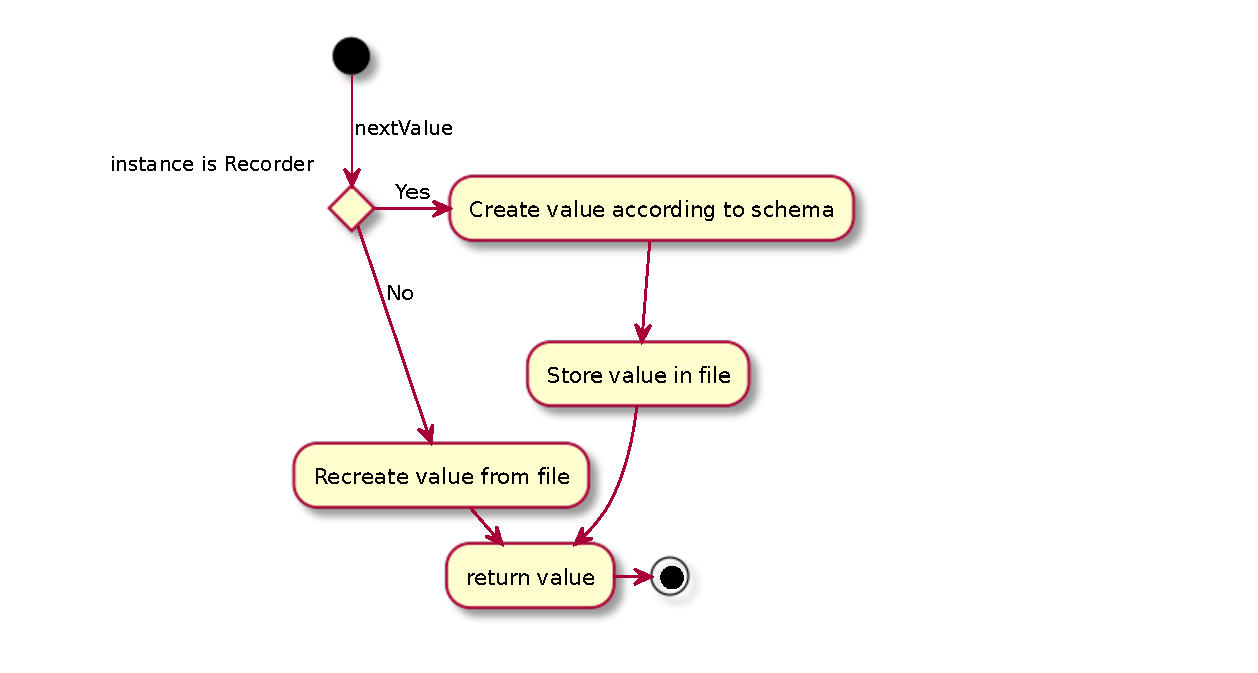
\includegraphics[width=.75\textwidth]{images/extensions/generalGeneratorWorkflow}
  \caption{Generic activity diagram showing how the generators will work.}
  \label{fig:generalGeneratorWorkflow}
\end{figure}

\section{Execution Tool}
\label{ch:design:se:executionTool}
YCSB has a script to run one workload on one database.
We have many workloads and multiple databases,
therefore it would save us a lot of time during evaluation,
if all workloads were executed on all databases sequentially.

That could be implemented as a script that takes the databases and their parameters together with the workload description files and executes one after another.
The results should be saved in a specified folder.

\section{Evaluation Tool}
\label{ch:design:se:evaluationTool}
To gather the results another script should iterate through the result folders of each database and workload and collect the results in a file for further evaluation.
